\documentclass[../elettronica]{subfiles}

\begin{document}
%Lezione 7

\section{Transistore bipolare a giunzione BJT}
\begin{figure}[h]
    \centering
    \begin{circuitikz}[scale=1.5]
        \draw
        (0, 0) to[diode, v=$V_{BC}$, i<=$I_C$] (2, 0) node[above]{$C$}
        (0, 0) to[diode, v=$V_{BE}$, i=$I_E$] (-2, 0) node[above]{$E$}
        (0, 0) to[short, i<=$I_B$] (0, -1) node[right]{$B$}

        (0, 0) node[circ]{}
        ;
    \end{circuitikz}
    \caption{transistor bipolare}
    \label{circit:transistor_bjt}
\end{figure}
\subsection{Modello di Ebers e Moll}
Supponiamo che $V_{BE} > 0$ e $V_{BC} < 0$. Questo ci permetterà di dire che il diodo tra base
ed emettitore è polarizzato in regione diretta ed il diodo tra base e collettore è polarizzato
in inversa.
Questo comporta che $I_E > 0$ e $I_C \approx 0$ e, considerando la legge di Kirchoff $I_B + I_C = I_E$,
abbiamo $I_B \approx I_E$.

Quello che accade se la distanza tra i due diodi è ridotta (che indicheremo con $w$), l'interazione tra
le loro cariche porta fa cambiare loro comportamento radicalmente, portando a far valere le
relazioni $I_e \approx -I_c$ e $I_b \approx 0$.


Quando $w$ è sufficientemente piccolo, quello che accade è che nel momento in cui il diodo tra base ed emettitore è' polarizzato
in diretta, ed il diodo tra base e collettore è polarizzato in inversa, la corrente fluisce prevalentemente fra collettore
ed emettitore a fronte di una corrente di base molto più piccola rispetto alle altre due regioni.
% 9:40

\begin{wrapfigure}{r}{.4\textwidth}
    \centering
    \vspace{-2\baselineskip}
    \begin{circuitikz}[/tikz/circuitikz/bipoles/length=1cm]
        \draw
        (0, 0)
        to[short, i=$\I{BC}$] (0.7, 0)
        to[diode] (2, 0)
        to[short, i<=$\I{C}$] ++(0.5, 0) node[below]{$C$}
        (0, 0)
        to[short, i=$\I{BE}$] (-0.7, 0)
        to[diode] (-2, 0)
        to[short, i=$\I{E}$] ++(-0.5, 0) node[above]{$E$}
        (0, 0) to[short, i<=$\I{B}$] (0, -1) node[right]{$B$}

        (0, 0) node[circ]{}
        ;
        \draw[clr-main-red] (2, 0)
        to[short, i=${\I{t}}$, color=clr-main-red] (2, 1)
        to[american controlled current source, color=clr-main-red] (-2, 1)
        -- (-2, 0)
        ;

        \draw[clr-primary] (-2, 1)
        -- (-2, 1.8)
        to[american controlled current source, color=clr-primary] ++(4, 0)
        -- (2, 1)
        ;
    \end{circuitikz}
\end{wrapfigure}
\vspace{10pt}
Possiamo tenere conto di questo comportamento attraverso un generatore aggiuntivo di corrente (riportato in rosso) che aggiunga
alla corrente prevista dal modello del diodo polarizzata in inversa, correntemente trascurabile, una nuova corrente
che dipende a sua volta esponenzialmente da \vbe. Chiameremo questa corrente $I_t$: corrente dell'\textbf{effetto transistore}.

\vspace{20pt}
\begin{tcolorbox}[title={Equazioni caratteristiche transistore}, width=\textwidth]
    \begin{align*}
        &\I{BE} = \diodecurrent[\I{BES}]{\V{BE}}\\
        &\I{BC} = \diodecurrent[\I{BCS}]{\V{BC}}\\
        &\I{t} = {\color{clr-main-red} \diodecurrent[\I{S}]{\V{BE}}} - {\color{clr-primary} \diodecurrent[\I{S}]{\V{BC}}}
    \end{align*}
\end{tcolorbox}

\vspace{10pt}
\noindent È semplice calcolare l'espressione della corrente di emettitore $\I{E}$, di collettore $\I{C}$ e di base $\I{B}$,
attraverso le equazioni di Kirchoff ai tre nodi.
Bisogna considerare che abbiamo utilizzato solo una particolare condizione di polarizzazione.
Se studiassimo il caso opposto, ovviamente otterremmo risultati simmetrici: vedremo che con $\V{BE} < 0$ e $\V{BC} > 0$
avremo una componente aggiuntiva di corrente ad effetto transistore, diretta in direzione opposta, rappresentabile anch'essa
con un generatore di corrente pilotato.

%17:39
\begin{tcolorbox}[title=Equazioni caratteristiche transistore (linearm. dipendenti)]
    \begin{align*}
        &\I{B} = \diodecurrent[\I{BES}]{\V{BE}} - \diodecurrent[\I{BC}]{\V{BC}}\\
        &\I{E} = \diodecurrent[(\I{S} + \I{BE})]{\V{BE}} - \diodecurrent[\I{S}]{\V{BC}}\\
        &\I{C} = \diodecurrent[\I{S}]{\V{BE}} - \diodecurrent[(\I{S} + \I{BCS})]{\V{BC}}\\
    \end{align*}
\end{tcolorbox}

\vspace{20pt}
\begin{wrapfigure}{r}{.2\textwidth}
    \vspace{-2\baselineskip}
    \begin{center}
        \begin{circuitikz}
            \draw (0, 0) node[npn](bjt){}
            (bjt.B) node[ocirc]{} node[left]{B}
            (bjt.E) node[ocirc]{} node[below]{E}
            (bjt.C) node[ocirc]{} node[above]{C}
            ;
        \end{circuitikz}
    \end{center}
    \caption{transistor npn}
    \label{component:transistor_npn}
\end{wrapfigure}

\noindent Il transistore in figura \ref{component:transistor_npn} prevede due giunzioni ed ha il nome di \textbf{transistore npn}.
Esiste anche il suo duale, \textbf{transistore pnp} al quale faremo solo un rapido cenno più avanti ma suo
comportamento è del tutto identico a quello che stiamo discutendo.

Per la legge di Kirchoff abbiamo se conosciamo due tra le differenze di potenziale ai lati del transistore, la terza è
univocamente determinata. Ragionamento del tutto analogo vale per le correnti.

Per determinare completamente il regime di funzionamento del transistore, occorre determinare le 6 grandezze: 3 correnti e 3
tensioni, attraverso 6 equazioni, due delle quali sono quelle di Kirchoff appena indicate.
Per trovare le altre quattro equazioni, utilizziamo lo stesso metodo che abbiamo applicato per determinare le
equazioni del diodo: mettiamo un morsetto a terra e, fornendo un potenziale su uno dei due morsetti rimanenti, misuriamo
il potenziale sull'ultimo morsetto.

Ovviamente è possibile connettere il transistor in 3 modi differenti: emettitore, base e collettore comune. Ma di queste
ultime due ce ne occuperemo più avanti.

\begin{figure}[h]
    \centering
    \begin{circuitikz}[scale=1.2]
        \draw (0, 0)
        to[american voltage source, v=$V_i$, i=$\I{B}$] (0, 2)
        -- (1, 2)
        -- (1, 1) node[npn, anchor=B](tr){}

        (tr.E) -- (tr.E |- 0, 0)
        (0, 0) -- (tr.E |- 0, 0)
        -- ++(1, 0) coordinate(x)

        (tr.C) -- (tr.C |- 0, 2)
        -- ++(1, 0)
        to[R, v^=$V_u$, i<=$\I{C}$] (x)
        ;
    \end{circuitikz}
    \caption{Connessione a Emettitore comune}
    \label{circuit:transistor_bjt_common_e}
\end{figure}

%37:00
\noindent Già osservando il circuito, possiamo notare che due incognite sono eliminate dalla equazione della tensione in ingresso
$\V{i} = \V{BE}$, che possiamo considerare data, e dall'equazione $\V{u} = R\cdot \I{C}$.
Ricordando che la corrente in ingresso corrisponde alla corrente di base, e che la corrente in uscita corrisponde alla
corrente di collettore, per le ultime due equazioni residue possiamo utilizzare quelle fornite dalle caratteristiche del transistore
elencate precedentemente.

\vspace{10pt}
\begin{tcolorbox}
    \begin{align*}
        &\I{B}(\V{BE}, \V{CE}) = \diodecurrent[\I{BES}]{\V{BE}} - \diodecurrent[\I{BC}]{\V{BC}}\\
        &\I{C}(\V{BE}, \V{CE}) = \diodecurrent[\I{S}]{\V{BE}} - \diodecurrent[(\I{S} + \I{BCS})]{\V{BC}}\\
    \end{align*}
\end{tcolorbox}
\vspace{10pt}
Siccome queste relazioni di correnti sono due funzioni di due variabili ($\V{BE}$ e $\V{CE}$), è necessario
un grafico in tre dimensioni per poterle rappresentare graficamente, e ciò non sarebbe pratico.

Per questo motivo riconduciamo queste espressioni ad una rappresentazione più semplice, riconducendoci ad una famiglia di curve parametriche
ponendo $\V{CE}$ come variabile indipendente e tracciando le funzioni al variare di $\V{CE}$ (Figura \ref{graph:transistor_bjt_3d}).

\newpage
\begin{figure}[h]
\begin{minipage}{.47\textwidth}
    \centering
    \def\vt{1}
    \def\kuno{0.001}
    \def\kdue{20}
    \begin{tikzpicture}[declare function={
            ib(\vbe,\vce) = \kuno *(e^(\vbe/\vt)-1) + \kdue *(e^((\vbe - \vce)/\vt -1));
        }]

        \begin{axis}[restrict y to domain=-1:10, ymin=-1, xmin=-1, xlabel=$\V{BE}$, ylabel=$\I{B}$]
            \foreach \i in {4, 4.250, ..., 6}{
                \addplot {ib(x, \i)};
            }

            \draw[->, thick] (4.5, 0.5) -- (2, 2) node[above]{$\V{CE}$};
            \draw
                (0.8, 0.4) node[above]{OFF}
                (4.3, 0.9) node[right] {AD}
                (3.5, 4.5) node[left]{SAT};
        \end{axis}
    \end{tikzpicture}
    \caption{$\I{B}(\V{BE})$ al variare di $\V{CE}$}
    \label{graph:transistor_bjt_3d}
\end{minipage}
\begin{minipage}{.47\textwidth}
    \centering
    \def\vt{1}
    \def\kuno{1.250}
    \def\kdue{3}
    \begin{tikzpicture}[declare function={
            ib(\vbe,\vce) = \kuno *(e^(\vbe/\vt)-1) - \kdue *(e^((\vbe - \vce)/\vt -1));
        }]

        \begin{axis}[restrict y to domain=-1:10, ymin=-1, xmin=-1, xlabel=$\V{CE}$, ylabel=$\I{C}$]
            \foreach \i in {0.25, 0.50, ...,1.5}
            {
                \addplot {ib(\i, x)};
            }

            \draw[->, thick] (3, 0.2)--(3, 4.5)
                node[left]{$\V{BE}$};
            \draw
                (4.5, 4.5) node[above]{AD}
                (4.5, 0.3) node[above]{OFF}
                (1, 3.3) node[above]{SAT};
        \end{axis}
    \end{tikzpicture}
    \caption{$\I{C}(\V{CE})$ al variare di $\V{BE}$}
\end{minipage}
\end{figure}

\vspace{20pt}
\noindent Il transistor è composto da 2 diodi, ognuno polarizzabile in regione diretta o regione inversa. Possiamo riconoscere quindi
quattro regioni di funzionamento del transistore, dipendenti da $\V{BE}$ e $\V{BC}$.
\begin{itemize}
    \item BE on, BC off: Regione normale di funzionamento o regione di polarizzazione attiva diretta
    \item BE off, BC on: Regione di polarizzazione attiva inversa.
    \item BE off, BC off: Regione di interdizione, per brevità diremo che il transistore è spento
    \item BE on, BC on: Regione di saturazione.
\end{itemize}

\subsubsection{Regione Attiva Diretta}
Prendendo in considerazione la regione di funzionamento attiva diretta, considerando che $e^{\V{BE} / \V{T}} > e^{\V{BC}/{\V{T}}}$
siccome il primo termine è maggiore di 1 per $\V{BE} > 0$ ed il secondo minore di 1 per $\V{BC} < 0$, possiamo semplificare le relative
equazioni caratteristiche del transistore in
\begin{align*}
    &\I{C} = \diodecurrent[\I{s}]{\V{BE}}\\
    &\I{B} = \diodecurrent[\I{BEs}]{\V{BE}}\\
    &\I{E} = \diodecurrent[(\I{s} + \I{BEs})]{\V{BE}}
\end{align*}
Osserviamo che in questa regione, tutte le correnti assumono la forma di esponenziale traslata in funzione della sola tensione $\V{BE}$.
In questo caso particolare, il circuito in figura \ref{circuit:transistor_bjt_common_e}, la corrente in uscita $\I{c}$ non è una funzione della tensione
di uscita $\V{u} = \V{CE}$, quindi si comporta come un circuito generatore di corrente costante/controllata in funzione di $\V{i}$.

Inoltre, siccome tutte le correnti dipendono dallo stesso esponenziale, allora sono proporzionali tra loro
\[
    \frac{\I{C}}{\I{B}} = \frac{\I{s}}{\I{BEs}} = \beta_F
\]
Per analogo ragionamento $\I{E} = (\beta_F+1) \I{B}$, e $\I{C} = \frac{\beta_F}{\beta_F + 1}\I{E} = \alpha_F \I{E}$.
Con $\alpha_F$ viene definita l'\textit{efficienza di emettitore}: maggiore è la costante più la corrente di collettore assomiglia alla corrente di emettitore.
Quindi siccome $\alpha_F = \frac{\beta_F}{\beta_F + 1}$, maggiore è $\beta_F$, più $\alpha_F$ è vicina ad 1, e migliore è il transistore.

\subsubsection{Regione attiva inversa}
Per ragionamento analogo alla regione precedente, $\V{BE} < 0$ e $\V{BC} > 0$ ci porta a trascurare i termini in funzione di $\V{BE}$
\begin{align*}
    &\I{C} = -\diodecurrent[(\I{S} + \I{BCs})]{\V{BC}}\\
    &\I{B} = \diodecurrent[\I{BCs}]{\V{BC}}\\
    &\I{E} = -\diodecurrent[\I{s}]{\V{BC}}\\
\end{align*}
Indicando con $\beta_R = {\I{s}}/{\I{BCs}}$, abbiamo che
\begin{align*}
    &\I{E} = - \beta_R \I{B}\\
    &\I{C} = -(\beta_R + 1) \I{B}\\
    &\I{E} = \frac{\beta_R}{1 + \beta_R}\I{C} = \alpha_R \I{C}
\end{align*}
Il crescere di $\beta_R$ aumenta le prestazioni del transistore: $\alpha_R \approx 1$.
\\[1em]
Nota: \textit{F e B a pedice, indicano Forward e Reverse}

\subsubsection{Regione di interdizione}
$\V{BE} < 0$ e $\V{BC} < 0$ ci portano ad osservare che ciascuna delle espressioni esponenziali è trascurabile, quindi:
\begin{align*}
    &\I{C} = \I{BCs}\\
    &\I{B} = - \I{BEs} - \I{BCs}\\
    &\I{E} = \I{BEs}
\end{align*}
"Il modello non ha bisogno dell'aggiunta di un generatore controllato per essere descritto".

\subsubsection{Regione di saturazione}
$\V{BE} > 0$ e $\V{BC} > 0$ indica che nessun esponenziale è trascurabile. Tutte le correnti dipendono da entrambe le tensioni di funzionamento $\V{BE}$ e $\V{BC}$.

\newpage
\subsection{Analisi del circuito transistore BJT}
Utilizzando le approssimazioni appena ricavate nel circuito in figura \ref{circuit:transistor_bjt_common_e}

\begin{tcolorbox}[title=Regione attiva diretta, width=\textwidth]
    \begin{align*}
        &\vu = \vbe - \vbc > 0\\
        &\vu = -R\I{C} = -R \diodecurrent[\I{s}]{\vbe} < 0
    \end{align*}
\end{tcolorbox}

\noindent
Quindi il circuito non può funzionare in regione normale.
Modifichiamo quindi il circuito aggiungendo un generatore di tensione $\V{cc}$ tale che $\vu = \V{cc} - R\I{c} > 0$.
Mantenendo compatibilità con la prima ipotesi.

\begin{figure}[h]
    \centering
    \begin{circuitikz}[scale=1.2]
        \draw (0, 0)
        to[american voltage source, v=$V_i$, i=$\I{B}$] (0, 3)
        -- (1, 3)
        -- (1, 1.5) node[npn, anchor=B, scale=2](tr){}

        (tr.E) -- (tr.E |- 0, 0)
        node[ground]{}
        (0, 0) -- (tr.E |- 0, 0)
        -- ++(1, 0) coordinate(x)

        (tr.C) -- (tr.C |- 0, 3)
        -- ++(1, 0)
        node[circ] {} node[above] {$\vu$}
        to[R, i<=$\I{C}$] ++(0, -2)

        (x) to[american voltage source, v_=$\V{cc}$] ++(0, 1)

        ;
    \end{circuitikz}
\end{figure}
\noindent
Siccome ci siamo assicurati che il circuito funzioni in regione attiva diretta, verifichiamo ora se è possibile che tale
circuito funzioni in regione attiva inversa:

\begin{tcolorbox}[title=Regione attiva inversa]
    \begin{align*}
        &\vu = \vbe - \vbc < 0\\
        &\vu = \V{cc} - R\I{C} > 0
    \end{align*}
\end{tcolorbox}

\noindent
Abbiamo dimostrato quindi che questo circuito, corretto appositamente per farlo lavorare in regione attiva diretta,
non può lavorare in regione attiva inversa. Per funzionare in quest'ultima regione il generatore di tensione \V{cc} dovrebbe
avere una tensione negativa, per questo motivo per analizzare di questo circuito, consideriamo solo
tre regioni di funzionamento.

\noindent
\begin{minipage}{.49\textwidth}
    \begin{tcolorbox}[title=Regione di interdizione]
        \vspace{-1.5em}
        \begin{align*}
        &\I{C} = \I{BEs} \approx 0\\
        &\vu = \V{cc}\\
        &\vbe = \vi < 0\\
        &\vbc = \vi - \vu < 0
        \end{align*}
    \end{tcolorbox}
\end{minipage}
\begin{minipage}{.49\textwidth}
    \begin{tcolorbox}[title=Attiva diretta]
        \begin{align*}
        &\vbe = \vi > 0\\
        &\vu = \V{cc} - R \diodecurrent[\I{s}]{\vi}\\
        \end{align*}
    \end{tcolorbox}
\end{minipage}

\noindent
In regione di saturazione abbiamo che
\begin{align*}
    \I{C} = \frac{\V{cc} - \vce}{R}
\end{align*}
Ricordandoci che in figura \ref{graph:ramo_di_carico} abbiamo già calcolato una relazione che lega \I{C} e \vce.
Tracciamo l'equazione di $\I{C}$ appena trovata. Ciascuno dei punti di intersezione in tale figura, rappresenta
quindi il luogo dei punti soluzione di questa equazione.
Dal grafico quindi possiamo osservare che in regione di saturazione, la tensione di uscita continua a calare, ma
tende asintoticamente ad un valore appena maggiore di 0.

\newpage
\begin{figure}[h]
    \centering
    \begin{minipage}{.48\textwidth}
        \def\vt{1}
        \def\kuno{1.250}
        \def\kdue{3}
        \begin{tikzpicture}[declare function={
                ib(\vbe,\vce) = \kuno *(e^(\vbe/\vt)-1) - \kdue *(e^((\vbe - \vce)/\vt -1));
            }]

            \begin{axis}[restrict y to domain=-1:10, ymin=-1, xmin=-1, xlabel=$\V{CE}$, ylabel=$\I{C}$]
                \foreach \i in {0.25, 0.50, ...,1.5}
                {
                    \addplot {ib(\i, x)};
                }

                \addplot [solid] coordinates {(0, 3) (4, 0)};
                \draw (0, 3) node[circ]{} node[left]{$\frac{\V{cc}}{R}$}
                    (4, 0) node[circ]{} node[below]{$\V{cc}$};
                \draw[->, thick] (3, 0.2)--(3, 4.5)
                    node[left]{$\V{i}$};
            \end{axis}
        \end{tikzpicture}
        \label{graph:ramo_di_carico}
        \caption{Grafico con ramo di carico}
    \end{minipage}
    \begin{minipage}{.48\textwidth}
        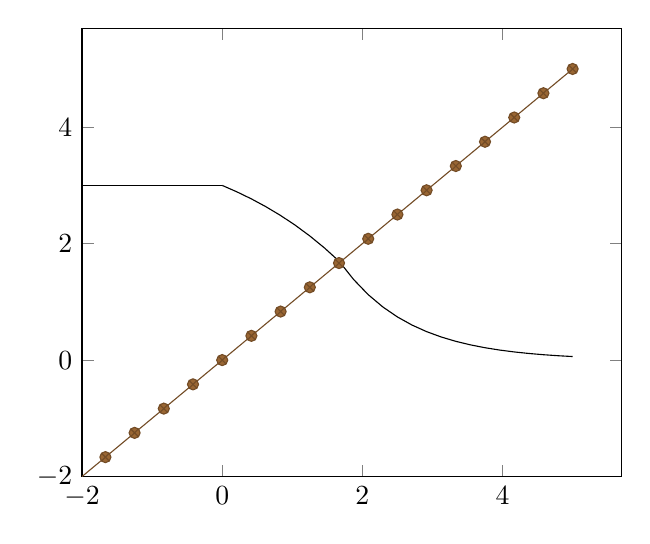
\begin{tikzpicture}[declare function={
                fun(\x,\R) = (3 - \R*(exp(\x/2) -1)) * (\x < (3 - \R*(exp(\x/2) -1)))
                + (\x > (3 - \R*(exp(\x/2) -1)))* (exp(-\x + 2.2));
            }]
            \begin{axis}[ymin=-2, xmin=-2]
                \addplot[domain=-5:0]{3};
                \addplot[domain=0:5]{fun(x, 1)};
                \addplot{x};
            \end{axis}
        \end{tikzpicture}
        \caption{Andamento qualitativo di \vu in funzione di \vi}
    \end{minipage}
\end{figure}

\noindent
In particolare, il valore a cui asintoticamente tende la tensione in uscita è dato da
\[
    \I{C} = \bjtcurrentic = 0
\]
Dove entrambi i termini 1 sono trascurabili, siccome entrambi gli esponenziali sono maggiori di 1.
\[
    \vce  = \V{T} \ln{\frac{1}{\alpha_R}}
\]
Quindi \vce è strettamente positivo, dato che $\alpha_R$ è compreso tra 0 ed 1, quindi il suo reciproco è maggiore di 1, e
rispettivo logaritmo è positivo.
Inoltre dato che questa espressione non dipende da \vbe, significa che tutte le caratteristiche intersecano l'asse delle ascisse
in corrispondenza di questo valore.
\end{document}
